\documentclass[../notes.tex]{subfiles}
\graphicspath{{\subfix{../figs/}}}

\begin{document}
% !TEX root = ../notes.tex

Good morning, everyone.
\begin{itemize}
	\item Homework \#10 is now due on Sunday at 11:59PM. Cool.
	\item There is a colloquium on complex dynamics at Evans 60, by Sarah Koch.
\end{itemize}

\subsection{The Mandelbrot Set}
Today we are talking about complex dynamics. Complex dynamics is the behavior of objects under iteration. As an example, we let $c\in\CC$ vary with the function
\[f_c(z)\coloneqq z^2+c.\]
For example, we might ask what happens to the point $0$ as we iterate it through $f_c$.
\begin{example}
	Fix $c=1$ so that $f_1(c)=z^2+1$. Then we compute
	\begin{align*}
		f_1(0) &= 1, \\
		f_1(1) &= 2, \\
		f_1(2) &= 5, \\
		f_1(5) &= 26.
	\end{align*}
	This is called ``blowing up'' because $0$'s iterations are to infinity.
\end{example}
It turns out that there are, roughly speaking, two options for the behavior of these iterations.
\begin{itemize}
	\item Perhaps $\left|f^{(n)}(0)\right|\to\infty$ as $n\to\infty$.
	\item Perhaps $\left|f^{(n)}(0)\right|$ is bounded.
\end{itemize}
To make this easier to compute, we have the following lemma.
\begin{lemma}
	Fix $c\in\CC$ and define $\{z_n\}_{n\in\NN}$ by $z_0\coloneqq0$ and $z_n\coloneqq f_c(z_{n-1})$ for $n>0$. If $|z_n|>2$ for any $n$, then $|z_n|\to\infty$ as $n\to\infty$.
\end{lemma}
\begin{proof}
	On one hand, take $|c|\le2$, we see that
	\[|z_{n+1}|\ge|z_n|^2-|c|>2|z_n|-2,\]
	so
	\[|z_{n+1}|-2>2(|z_n|-2)\]
	which goes to $\infty$ because it's constantly doubling. If $|c|>2$, one can do something similar.
\end{proof}
\begin{example}
	For $c=-1$, we have
	\[f_{-1}(0)=-1,\]
	which will simply repeat itself, which in particular is bounded.
\end{example}
We want to be able to do lots of computations, so we should use a computer. Here are the iterations for $z=0.39+0.2i$.
\begin{center}
	\begin{asy}
		unitsize(5cm);

		pair iter(pair z, pair c)
		{
			return (z.x*z.x - z.y*z.y + c.x, 2*z.x*z.y + c.y);
		}
		
		pair z = (0,0);
		pair c = (0.39,0.2);
		dot(z);
		
		path p = z;
		for(int i = 0; i < 30; ++i)
		{
			z = iter(z,c);
			p = p -- z;
		}
		draw(p);
		
		draw((-0.5,0) -- (0.75,0), arrow=EndArrow, p=dotted);
		draw((0,-0.25) -- (0,1), arrow=EndArrow, p=dotted);
		label("$\mathrm{Re}$", (1,0), E);
		label("$\mathrm{Im}$", (0,1), N);		
	\end{asy}
\end{center}
This path looks bounded.

The set of points $c$ for which this remains bounded has a name.
\begin{definition}[Mandelbrot set]
	The \textit{Mandelbrot set} is the set of all $c\in\CC$ such that
	\[\left\{f_c^{(n)}(0):n\in\NN\right\}\]
	is bounded.
\end{definition}
\begin{remark}
	The Mandelbrot set is named by Benoit B. Mandelbrot.
\end{remark}
\begin{remark}
	The ``B'' in Benoit B. Mandelbrot stands for ``Benoit B. Mandelbrot.''
\end{remark}
If we color all the points $c$ for which we remain bounded, we get the following figure. (The graphics were created with Asymptote.)
\begin{center}
	
\includegraphics[scale=0.8]{mandelbrot.png}
	% unitsize(5cm);
	% pair iter(pair z, pair c)
	% {
	% 	return (z.x*z.x - z.y*z.y + c.x, 2*z.x*z.y + c.y);
	% }
	% bool test(pair c)
	% {
	% 	pair z = (0,0);
	% 	real m = 0;
	% 	for(int i = 0; i < 50; ++i)
	% 	{
	% 		z = iter(z, c);
	% 		m = z.x*z.x + z.y*z.y;
	% 		if(m > 2)
	% 			return false;
	% 	}
	% 	return true;
	% }
	% real res = 0.002;
	% for(real a = -2; a <= 1; a += res)
	% {
	% 	for(real b = 0; b <= 2; b += res)
	% 	{
	% 		if(test((a,b)))
	% 		{
	% 			filldraw(shift(a, b) * scale(res*0.9) * unitsquare);
	% 		}
	% 	}
	% }
	% add(reflect((-2.25, 0), (0.75, 0)) * currentpicture);
\end{center}
This is more fun to Zoom it; here we have zoomed in to $z=0.25$.
\begin{center}
	
\includegraphics{zoom.png}
	% unitsize(16cm);
	% pair iter(pair z, pair c)
	% {
	% 	return (z.x*z.x - z.y*z.y + c.x, 2*z.x*z.y + c.y);
	% }
	% bool test(pair c)
	% {
	% 	pair z = (0,0);
	% 	for(int i = 0; i < 20; ++i)
	% 	{
	% 		z = iter(z, c);
	% 		if(z.x*z.x + z.y*z.y > 2)
	% 			return false;
	% 	}
	% 	return true;
	% }
	% for(real a = 0; a <= 0.5; a += 0.003)
	% {
	% 	for(real b = -0.25; b <= 0.25; b += 0.003)
	% 	{
	% 		if(test((a,b)))
	% 		{
	% 			filldraw(shift(a, b) * scale(0.003) * unitsquare);
	% 		}
	% 	}
	% }
\end{center}
There are fun things that we can say about the Mandelbrot set, even though it looks very strange.
\begin{theorem}
	The Mandelbrot set is connected.
\end{theorem}
The proof is about 200 pages, in French, like all good mathematics.
\begin{remark}
	It is conjectured that the Mandelbrot set is ``locally connected''---every point has a connected neighborhood.
\end{remark}

\subsection{Julia Sets}
One might ask what happens if we fix $c$ and then let the starting point $z$ vary instead. This gives the following definition.
\begin{definition}[Julia set]
	Fix $c$. Then the set
	\[\left\{x\in\CC:\left|f^{(n)}_c(x)\right|\text{ is bounded as }n\to\infty\right\}\]
	is the \textit{filled Julia set of $c$}.
\end{definition}
\begin{remark}
	Gaston Julia, for whom Julia sets are named after, is often pictured wearing a mask because he lost his nose in World War I.
\end{remark}
\begin{example}
	Fix $c=0$ so that we are looking at $f^{(n)}(z)=z^{2^n}$. Then we can see that the Julia set is just $\overline{B(0,1)}$---everything outside here will have exploding norm, and certainly $|z|\le1$ implies $\left|z^{2^n}\right|\le1$.
\end{example}
Connectivity of Julia sets is a somewhat strange phenomenon. Here is the filled Julia set for $c=0.25$.
\begin{center}
	
\includegraphics[scale=0.8]{julia0.25+0i.png}
\end{center}
And here is the filled Julia set for $c=0.26$.
\begin{center}
	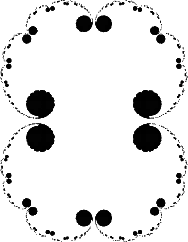
\includegraphics[scale=0.8]{julia0.26+0i.png}
	% unitsize(4cm);
	% pair iter(pair z, pair c)
	% {
	% 	return (z.x*z.x - z.y*z.y + c.x, 2*z.x*z.y + c.y);
	% }
	% bool test(pair c, pair z)
	% {
	% 	real m = 0;
	% 	for(int i = 0; i < 50; ++i)
	% 	{
	% 		z = iter(z, c);
	% 		m = z.x*z.x + z.y*z.y;
	% 		if(m > 2)
	% 			return false;
	% 	}
	% 	return true;
	% }
	% pair c = (0.24,0);
	% real res = 0.003;
	% for(real a = -2; a <= 2; a += res)
	% {
	% 	for(real b = -2; b <= 2; b += res)
	% 	{
	% 		if(test(c, (a,b)))
	% 		{
	% 			filldraw(shift(a, b) * scale(res) * unitsquare);
	% 		}
	% 	}
	% }
\end{center}
So indeed, connectivity looks sporadic, in some sense. Here is an amazing result.
\begin{theorem}
	The Mandelbrot set is precisely the values of $c\in\CC$ so that the filled Julia set of $c$ is connected.
\end{theorem}
In general, dynamics questions are somewhat easy to state but very hard to answer. Here is an example.
\begin{definition}
	A complex number $z\in\CC$ is \textit{preperiodic} for a polynomial $f(z)\in\CC[z]$ if and only if there are distinct $m$ and $n$ so that
	\[f^{(m)}(z)=f^{(n)}(z).\]
\end{definition}
The image here is that the points should ``loop'' in on themselves, in some sense. And here is our result.
\begin{theorem}
	Fix an integer $d\ge2$ and complex numbers $a,b\in\CC$. Then the set of parameters $c\in\CC$ such that both $a$ and $b$ are preperiodic for the polynomial $f(z)\coloneqq z^d+c$ is infinite if and only if $a^d=b^d$.
\end{theorem}
This is a really hard result, proven in roughly the last decade.
\end{document}